\documentclass[11pt, a4paper]{article}
\usepackage[utf8]{inputenc}
\usepackage[IL2]{fontenc}
\usepackage[left=2cm,top=3cm, text={17cm, 24cm}]{geometry}
\usepackage[czech]{babel}
\title{ITY2}
\author{xhudak03}
\date{March 2021}
\usepackage{amsmath, amsthm, amssymb}
\usepackage{times}
\usepackage{multirow}
\usepackage[ruled,noline,longend, czech,linesnumbered]{algorithm2e}
\usepackage{graphicx}
\usepackage{picture}
\usepackage{rotating}
\usepackage{pdflscape}
\usepackage[flushmargin]{footmisc}
\usepackage{url}


\begin{document}
\begin{titlepage}
\begin{center}
{\Huge
\textsc{Vysoké učení technické v Brně\huge{\\[0.4em]Fakulta informačních technologií}}}\\
\vspace{\stretch{0.382}}
\LARGE
Typografie a publikování -- 3. projekt\\[0.3em]\Huge Tabulky a obrázky
\vspace{\stretch{0.618}}
\end{center}
{\LARGE 22. března 2021 \hfill
David Hudák}
\thispagestyle{empty}
\end{titlepage}

\clearpage
\pagenumbering{arabic} 
\newpage

\section{Úvodní strana}

Název práce umístěte do zlatého řezu a nezapomeňte uvést dnešní datum a vaše jméno a příjmení.

\section{Tabulky}
Pro sázení tabulek můžeme použít buď prostředí \verb|tabbing| nebo prostředí \verb|tabular|.

\subsection{Prostředí \texttt{tabbing}}
Při použití \verb|tabbing| vypadá tabulka následovně:

\begin{tabbing}
    \hspace{1in} \= \hspace{0.45in} \= \hspace{0.5in}\kill 
     \textbf{Ovoce} \>\textbf{Cena} \quad\>\textbf{Množství}  \\
     Jablka \> 25,90 \> 3 kg \\
     Hrušky \> 27,40 \> 2,5 kg \\
     Vodní melouny \> 35,– \> 1 kus
\end{tabbing}
Toto prostředí se dá také použít pro sázení algoritmů, ovšem vhodnější je použít 
prostředí \verb|algorithm| nebo \verb|algorithm2e| (viz sekce \ref{sekce3}).

\setlength{\skip\footins}{1cm}
\subsection{Prostředí \texttt{tabular}}
Další možností, jak vytvořit tabulku, je použít prostředí \verb|tabular|. Tabulky pak 
budou vypadat takto\footnote{\indent Kdyby byl problem s \texttt{cline}, zkuste se podívat třeba sem: 
http://www.abclinuxu.cz/tex/poradna/show/325037}:

\catcode`\-=12
\begin{table}[h]
    \centering
\begin{tabular}{|c|c|c|}
    \hline
     & \multicolumn{2}{|c|}{\bfseries Cena}  \\
     \cline{2-3}
    
    \textbf{Měna} & \textbf{nákup} & \textbf{prodej} \\
    \hline
    EUR & 25,227 & 26,943 \\
    GBP & 29,368 & 31,492 \\
    USD & 21,260 & 22,661 \\
    \hline
    
\end{tabular}
\caption{Tabulka kurzů k dnešnímu dni}
\label{tab:my_label}
\end{table}

\begin{table}[h]
    \centering
    \begin{tabular}{|c|c|}
        \hline
        $A$ & $\neg A$  \\
        \hline
         \textbf{P}& N \\
         \hline
         \textbf{O}& O \\
         \hline
         \textbf{X} & X \\
         \hline
         \textbf{N} & P \\
         \hline
    \end{tabular}
    \begin{tabular}{|c|c|c|c|c|c|}
    \hline
        \multicolumn{2}{|c|}{\multirow{2}{*}{\bfseries $A \wedge B$}} &
        \multicolumn{4}{|c|}{B}\\
        \cline{3-6}
         \multicolumn{2}{|c|}{} & \textbf{P} & \textbf{O} & \textbf{X} & \textbf{N} \\
         \hline
         \multirow{4}{*}{A} & \textbf{P} & P & O & X & N\\
         \cline{2-6}
         & \textbf{O} & O & O & N & N\\
         \cline{2-6}
         & \textbf{X} & X & N & X & N\\
         \cline{2-6}
         & \textbf{N} & N & N & N & N\\
         \cline{1-6}
    \end{tabular}
    \begin{tabular}{|c|c|c|c|c|c|}
    \hline
        \multicolumn{2}{|c|}{\multirow{2}{*}{\bfseries $A \lor B$}} &
        \multicolumn{4}{|c|}{B}\\
        \cline{3-6}
         \multicolumn{2}{|c|}{} & \textbf{P} & \textbf{O} & \textbf{X} & \textbf{N} \\
         \hline
         \multirow{4}{*}{A} & \textbf{P} & P & P & P & P\\
         \cline{2-6}
         & \textbf{O} & P & O & P & O\\
         \cline{2-6}
         & \textbf{X} & P & P & X & X\\
         \cline{2-6}
         & \textbf{N} & P & O & X & N\\
         \cline{1-6}
    \end{tabular}
    \begin{tabular}{|c|c|c|c|c|c|}
    \hline
        \multicolumn{2}{|c|}{\multirow{2}{*}{\bfseries $A \to B$}} &
        \multicolumn{4}{|c|}{B}\\
        \cline{3-6}
         \multicolumn{2}{|c|}{} & \textbf{P} & \textbf{O} & \textbf{X} & \textbf{N} \\
         \hline
         \multirow{4}{*}{A} & \textbf{P} & P & O & X & N\\
         \cline{2-6}
         & \textbf{O} & P & O & P & O\\
         \cline{2-6}
         & \textbf{X} & P & P & X & X\\
         \cline{2-6}
         & \textbf{N} & P & P & P & P\\
         \cline{1-6}
    \end{tabular}
    \caption{Protože Kleeneho trojhodnotová logika už je \uv{zastaralá}, uvádíme si zde příklad čtyřhodnotové logiky.}
    \label{tab:my_label2}
\end{table}

\newpage
\section{Algoritmy} \label{sekce3}

Pokud budeme chtít vysázet algoritmus, můžeme použít prostředí 
\verb|algorithm|\footnote{\indent Pro nápovědu, jak zacházet s prostředím algorithm, můžeme zkusit tuhle stránku:\\
http://ftp.cstug.cz/pub/tex/CTAN/macros/latex/contrib/algorithms/algorithms.pdf.} nebo \verb|algorithm2e|\footnote{\indent Pro algorithm2e zase tuhle:
http://ftp.cstug.cz/pub/tex/CTAN/macros/latex/contrib/algorithm2e/algorithm2e.pdf.}.
\mbox{Příklad}~použití prostředí \verb|algorithm2e| viz Algoritmus \ref{alg:algoritmus}.
\\\\\\
\IncMargin{1.5em}
\begin{algorithm}[H]
\label{alg:algoritmus}
\SetNlSty{textbf}{}{:}
\SetAlgoLined
\Indm
\SetKwInput{KwInput}{Input} 
\KwInput{($X_{t-1}$, $u_t$, $z_t$)}
    
\SetKwInput{KwOutput}{Output} 
\KwOutput{$X_t$}
\Indp
\BlankLine
$\overline{X_t} = X_t = 0$
\SetAlgoNoLine

\For{$k=1$ \textnormal{to} $M$}{
    $x_t^{[k]} = sample\_motion\_model(u_t, x^{[k]}_{t-1})$
    
    $\omega_t^{[k]}=measurement\_model(z_t, x_t^{[k]}, m_{t-1})$
    
    $m_t^{[k]} = updated\_occupancy\_grid(z_t, x_t^{[k]}, m_{t-1}^{[k]})$
    
    $\overline{X_t} = \overline{X_t} + \langle x_x^{[m]}, \omega_t^{[m]}\rangle$
    
}

\For{$k=1$ \textnormal{to} $M$}{
    draw $i$ with probability $\approx \omega_t^[i]$
    
    add $\langle x_x^{[k]}, m_t^{[k]} \text{to} X_t \rangle$
}

\Return $X_t$


    
\caption{\textsc{FastSLAM}}
\end{algorithm}
\DecMargin{1.5em}
\section{Obrázky}
Do našich článků můžeme samozřejmě vkládat obrázky. Pokud je obrázkem fotografie,
můžeme klidně použít bitmapový soubor. Pokud by to ale mělo být nějaké schéma nebo
něco podobného, je dobrým zvykem takovýto obrázek vytvořit vektorově.

\begin{figure}[h]
    \centering
    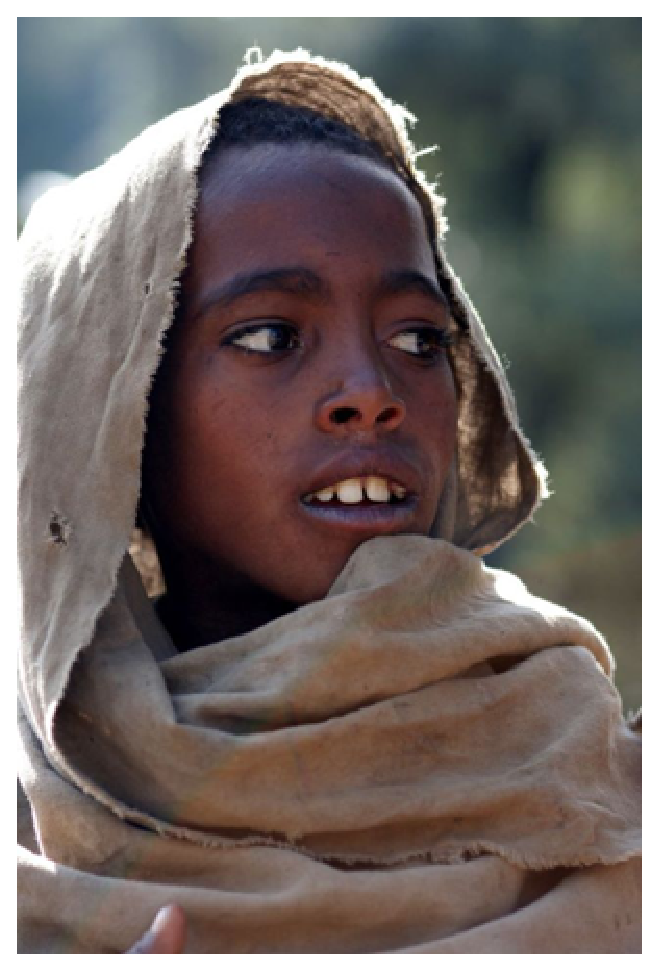
\includegraphics[scale=0.4]{etiopan.eps}
    \reflectbox{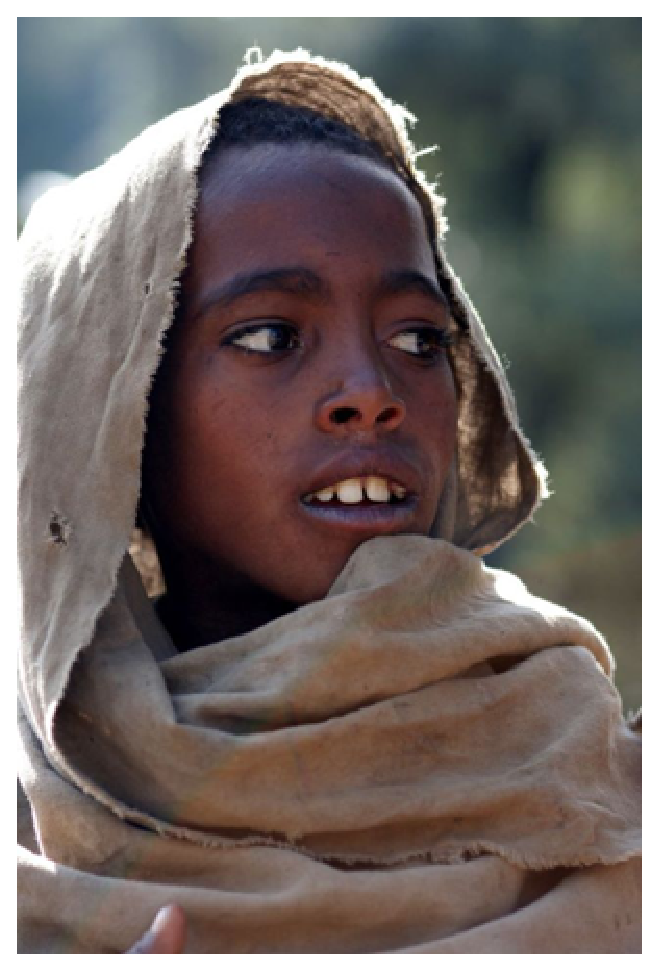
\includegraphics[scale=0.4]{etiopan.eps}}
    \caption{Malý Etiopánek a jeho bratříček}
    \label{fig:my_label3}
\end{figure}

\newpage
Rozdíl mezi vektorovým \ldots
\begin{figure}[h]
    \centering
    
\includegraphics[scale=0.4]{oniisan.eps}
    \caption{Vektorový obrázek}
    \label{fig:my_label4}
\end{figure}
\\
\noindent\ldots  a bitmapovým obrázkem
\begin{figure}[h]
    \centering
    
\includegraphics[scale=0.6]{oniisan2.eps}
    \caption{Bitmapový obrázek}
    \label{fig:my_label5}
\end{figure}

\noindent se projeví například při zvětšení.

Odkazy (nejen ty) na obrázky \ref{fig:my_label3}, \ref{fig:my_label4} a \ref{fig:my_label5}, na  
tabulky \ref{tab:my_label} a \ref{tab:my_label2} a také na algoritmus \ref{alg:algoritmus} jsou udělány pomocí 
křížových odkazů. Pak je ovšem potřeba zdrojový soubor přeložit dvakrát.

Vektorové obrázky lze vytvořit i přímo v \LaTeX u, například pomocí
prostředí \verb|picture|.
\newpage
\setlength{\unitlength}{1cm}
\thicklines
\begin{landscape}
\begin{figure}
    \centering
    \setlength{\unitlength}{1cm}
    \begin{picture}(20cm,11cm)
    
    \linethickness{1pt}
        \put(0,0){\line(1,0){20}}
        \put(20,0){\line(0,1){11}}
        \put(20,11){\line(-1,0){20}}
        \put(0,11){\line(0,-1){11}}
    \linethickness{4pt}
        \put(1,1){\line(1,0){18}}
    \linethickness{1.5pt}
        \put(17,8){\circle{}}
        \put(2,1){\line(1,1){8}}
        \put(10,9){\line(1,-1){8}}
    \linethickness{1pt}
        \put(9,8){\line(1,0){2}}
        \put(7,6){\line(1,0){6}}
        \put(5,4){\line(1,0){10}}
    % \linethickness{1pt} - z architektonických důvodů byla ponechána pro 
    % dveře šíře jednoho bodu
        \put(11,1){\line(0,1){1.75}} 
        \put(11,2.75){\line(1,0){2}}
        \put(13,2.75){\line(0,-1){1.75}}
        \put(5,1.5){\line(0,1){1}}
        \put(5,2.5){\line(1,0){2}}
        \put(7,2.5){\line(0,-1){1}}
        \put(7,1.5){\line(-1,0){2}}
        \put(7,6){\line(-1,1){5}}
        \put(6,7){\line(-1,0){6}}
        \put(4,3){\line(-1,0){4}}
        \end{picture}
    \caption{Skutečně moderní bydlení pro mě a mého kocoura Kryšpína v rušném sousedství velkoměsta.}
    \label{fig:my_label}
\end{figure}

\end{landscape}


\end{document}

